\chapter{数值计算}
\label{ch:numerical}

\gls*{ml}算法通常需要大量的数值计算。这通常指那些解决数学问题的算法,这样的算法使
用的方法是通过一个迭代的过程,而不是给定一个对正确解的象征性的表达式分析导出一个
公式。常见的操作包括优化(找到一个参数的值,最小化或者最大化一个函数)和解线性方
程组。当函数涉及到实数,在一个计算机上即使只是对一个数学函数求值都是困难的,它无
法用有限内存精确表示。

\section{溢出和下溢}
\label{sec:overflow_and_underflow}

在一个数字计算机上做连续的数学计算的主要困难,是我们需要用一个有限的、以 bit 位的
模式的数字来表示无限多的实数。这意味着对于几乎所有的实数,当我们在计算机中表示这
些数字时引起了一些近似误差。在多数情况下,这仅仅是舍入误差。舍入误差是有问题的,
尤其是当它经过许多操作后进一步恶化,并且,如果算法没有被设计为最小化舍入误差的累
加,它们能使理论上可行的算法在实际中失败。

一种特别严重的舍入误差的形式是\emph{\gls{underflow}}。\gls*{underflow}发生在当数
字接近 $0$ 而被舍入为 $0$ 的时候。许多函数当它们的参数为 $0$ 而不是一个小的正数时
表现出本质上的不同。例如,我们通常想要避免被 $0$ 除(当这种情况发生时有些软件环境
会产生异常,其它的会返回结果为一个占位符 \verb!not-a-number! 的值)或者取 $0$ 的
对数(这通常被当作 $-\infty$ 对待,如果它被用于更进一步的算数操作会变
成 \verb!not-a-number!)。

另一个有高度破坏性的数值误差的形式是\emph{\gls{overflow}}。\gls*{overflow}发生在
当具有大的数量级的数字被近似为 $\infty$ 或 $-\infty$ 的时候。进一步的算数计算通常
把这些无限值改为 \verb!not-a-number! 值。

一个函数必须针对\gls*{underflow}和\gls*{overflow}稳定化的函数是\gls*{softmax}函
数。\gls*{softmax}函数常常被用于预测和一个多项分布关联的概率。\gls*{softmax}函数
被定义为
\begin{equation}
  \mathrm{softmax}(\pmb{x})_i = \frac{\exp(x_i)}{\sum_{j=1}^n\exp(x_j)}
\end{equation}

考虑当所有的 $x_i$ 等于某个常数 $c$ 时会发生什么。通过分析,我们能够看到所有的输
出应该等于 $\frac{1}{n}$。从数字上看,当 $c$ 有很大的数量级时这可能不会发生。如
果 $c$ 是很小的负数,那么 $\exp(c)$ 会\gls*{underflow}。这意味着\gls*{softmax}的
分母会变成 $0$,所以最后的结果是未定义的。当 $c$ 是非常大的正
数,$\exp(c)$ 会\gls*{overflow},再一次导致整个表达式为未定义的。这两个困难都能够
通过对 $\mathrm{softmax}(\pmb{z})$ ~——~这里 $\pmb{z} = \pmb{x} - \max_ix_i$
~——~求值来解决。通过分析,简单的代数显示,将输入\gls*{vec}加上或者减去一个标
量,$\mathrm{softmax}$ 函数的值不会被改变。对 $\max_ix_i$ 做减法导致 $\exp$ 有最
大的参数而为 $0$,这排除了\gls*{overflow}的可能。同样地,分母中至少一项值为 $1$,
这排除了分母中导致被 $0$ 除的\gls*{underflow}的可能。

还有一个小问题。分子上的\gls*{underflow}仍然能引起整个表达式求值为 $0$。这意味着
如果我们通过先运行 $\mathrm{softmax}$ 子程序然后传递其结果给 $\log$ 函数来实
现 $\log\mathrm{softmax(\pmb{x})}$ 时,我们会错误地得到
$-\infty$。相反,我们必需实现一个单独的函数,它以一个在数值上稳定的方式计
算 $\log\mathrm{softmax}$。$\log\mathrm{softmax}$ 函数能够使用我们用于稳定
化 $\mathrm{softmax}$ 函数的相同技巧来被稳定。

在这本书中,对于大部分内容,我们没有明确地详细说明所有涉及到实现不同算法的数值上
的考虑。底层库的开发者应该在实现\gls*{dl}算法时把数值问题记在心里。本书的大部分读
者可以简单地依赖已经提供稳定实现的底层库。在有些情况下,有可能实现一个新的算法并
且自动让新的实现稳定化。Theano
\citep{bergstra+al:2010-scipy-small,Bastien-2012}是一个软件包的例子,它自动检测并
稳定化许多常见的、出现在\gls*{dl}环境中的、数值上不稳定的表达式。

\section{不合理的条件作用}
\label{sec:poor_conditioning}

条件作用是指一个函数如何随着它的输入中的微小变化快速改变。那些当它们的输入被微小
扰动时快速变化的函数可能对科学计算是有问题的,这是因为在输入中的舍入误差可以导致
输出上的巨大变化。

考虑函数 $f(\pmb{x}) = \pmb{A}^{-1}\pmb{x}$。当 $\pmb{A} \in \mathbb{R}^{n
  \times n}$ 有一个\gls*{eigen-val}分解,它的\emph{\gls{cond-num}}\,是
\begin{equation}
  \max_{i,j}|\frac{\lambda_i}{\lambda_j}|
\end{equation}

这是最大和最小幅度的\gls*{eigen-val}的比率。当这个数很大时,矩阵求逆对于输入中的
误差是特别敏感的。

这个敏感性是矩阵本身的一个本质特性,不是在矩阵求逆中舍入误差的结果。当我们用真的
逆矩阵相乘时,条件不合理的矩阵放大了预先存在的误差。在实践中,这个误差会被求逆过
程自身中的误差进一步加剧。

\section{基于梯度的最优化}
\label{sec:gradient-based_optimization}

大部分\gls*{dl}算法涉及到某种优化。优化是指通过改变 $\pmb{x}$ 来最小化或者最大化
某个函数 $f(\pmb{x})$ 的任务。我们通常以最小化 $f(\pmb{x})$ 的形式表达大部分优化
问题。最大化可以通过一个最小化 $-f(\pmb{x})$ 的算法来完成。

我们想要最小化或者最大化的函数被称
为\emph{\gls{obj-func}}\,或者\emph{\gls{criterion}}。当我们正在最小化它的时候,我
们也可能称它\emph{\gls{cost-func}},\emph{\gls{loss-func}},或
者\emph{\gls{err-func}}。尽管有些\gls*{ml}出版物给这些术语指定特别的意义,在这本
数中,我们交换使用这些术语。

我们常常用一个上标 $*$ 表示最小化或者最大化一个函数的值。例如,我们可能
说 $\pmb{x}^* = \arg\min f(\pmb{x})$。

我们假设读者已经熟悉微积分,但是这里提供了一个关于微积分概念如何和最优化相联系的
简要回顾。

假设我们有一个函数 $y = f(x)$,其中 $x$ 和 $y$ 都是实数。这个函数的导数被表示
为 $f'(x)$ 或者 $\frac{dy}{dx}$。导数 $f'(x)$ 给出了 $f(x)$ 在点 $x$ 的斜率。换句
话说,它指定了如何调整输入中的一个小的变化,以至于获得相应的输出中的变化:$f(x +
\epsilon) \approx f(x) + \epsilon f'(x)$。

\begin{figure}[h]
  \centering
  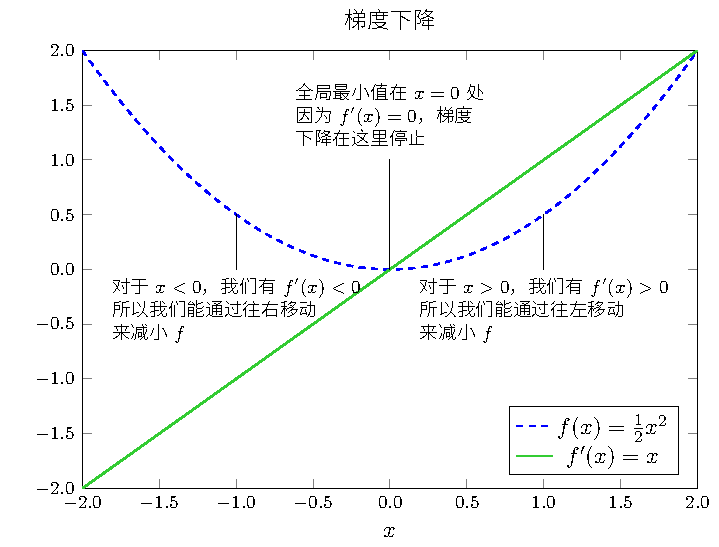
\includegraphics{gradient_descent}
  \caption{一个图例,演示一个函数的导数如何能够被用于沿着函数往下移动到一个最小值。
    这个技术被称为\emph{\gls{gradient-descent}}。\label{fig:gradient_descent}}
\end{figure}

导数对于最小化一个函数是非常有用的,因为它告诉我们如何改变 $x$ 以至于在 $y$ 上产
生一个小的改进。例如,我们知道对于足够小的 $\epsilon$,$f(x - \epsilon
\mathrm{sign}(f'(x)))$ 比 $f(x)$ 小。这样我们能够通过以导数的相反符号小步地移
动 $x$ 来减小
$f(x)$。这个技术被称为\emph{\gls{gradient-descent}}。这个技术的示例参见
图~\ref{fig:gradient_descent}。

当 $f'(x) = 0$ 时,导数没有提供关于往哪个方向移动的信息。在 $f'(x) = 0$ 的点被称
为\emph{\gls{critical-points}}\,或者\emph{\gls{stationary-points}}。一
个\emph{\gls{local-min}}\,是一个在 $f(x)$ 比所有相邻点都小的位置处的点,所以不再
可能通过做极小的步进来减小 $f(x)$。一个\emph{\gls{local-max}}\,是一个在 $(fx)$ 比
所有相邻点都大的位置处的点,所以不再可能通过做极小的步进来增加
$f(x)$。某些\gls*{critical-points}既不是最大值也不是最小值。它们被称
为\emph{\gls{saddle-points}}。每种类型的临界点参见图~\ref{fig:critical_points}。

\begin{figure}[h]
  \centering
  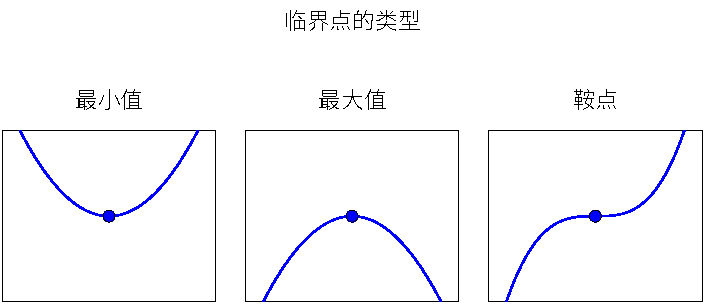
\includegraphics{critical_points}
  \caption{一维空间中三种临界点的示例。一个临界点是斜率为 $0$ 的点。这样的一个点
    既可以是一个局部最小值~——~它比相邻点更低,一个局部最大值~——~它比相邻点更高,
    也可以是一个鞍点~——~它有高于和低于这个点自身的相邻
    点。\label{fig:critical_points}}
\end{figure}

一个取得 $f(x)$ 的绝对最低值的点是一个\emph{\gls{global-min}}。函数可能存在只有一
个\gls*{global-min}或者多个\gls*{global-min}。也有可能存在并不是全局最优化的局部
最小值。在\gls*{dl}环境中,我们优化的函数可能有许多不是最优的局部最小值,而且许多
鞍点被非常平整的区域包围。所有这些使得最优化非常困难,尤其当函数的输入是多维的时
候。所以我们通常满足于找到一个非常低的 $f$ 的值,但不是必须在任何正式意义上是最小
的。参见图~\ref{fig:approximate_minimization} 的示例。

\begin{figure}[h]
  \centering
  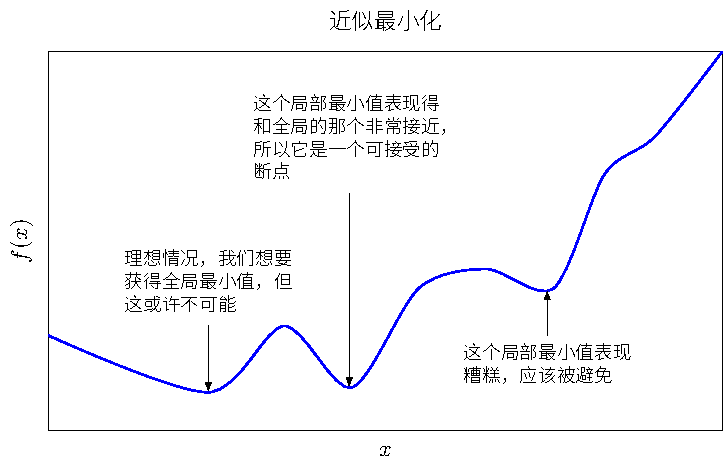
\includegraphics{approximate_minimization}
  \caption{最优化算法可能失败\label{fig:approximate_minimization}}
\end{figure}

我们常常最小化有多个输入的函数:$f: \mathbb{R}^n \rightarrow \mathbb{R}$。为了
让``最小化''的概念有意义,必须只有一个(标量)输出。

对于具有多个输入的函数,我们必须利用\emph{\gls{partial-derivatives}}\,的概念。偏
导数 $\frac{\partial}{\partial x_i}f(\pmb{x})$ 测量 $f$ 在点 $\pmb{x}$ 仅当变
量 $x_i$ 增加时如何改变。\emph{\gls{gradient}}\,概括了在导数是相对于一
个\gls*{vec}的情况下导数的概念:$f$ 的梯度是包含所有偏导数的\gls*{vec},表示
为 $\nabla_{\pmb{x}}f(\pmb{x})$。梯度中的元素 $i$ 是 $f$ 对于 $x_i$ 的偏导数。在
多维中,临界点是那些梯度中的每个元素等于 $0$ 的点。

$\pmb{u}$ 方向(一个单位\gls*{vec})上的\emph{\gls{directional-derivative}}\,是函
数 $f$ 在 $u$ 方向上的斜率。换句话说,方向导数是函数 $f(\pmb{x} +
\alpha\pmb{u})$ 对于 $\alpha$ 的导数,在 $\alpha = 0$ 处求值。使用这个链式规则,
我们能够看到
$\frac{\partial}{\partial\alpha}f(\pmb{x} + \alpha\pmb{u}) =
\pmb{u}^{\top}\nabla_{\pmb{x}}f(\pmb{x})$。

为了最小化 $f$,我们想要找到 $f$ 减小最快的方向。我们能够使用方向导数来这样做:
\begin{gather}
  \min_{\pmb{u},\pmb{u}^{\top}\pmb{u}=1}\pmb{u}^{\top}\nabla_{\pmb{x}}f(\pmb{x})\\
  = \min_{\pmb{u},\pmb{u}^{\top}\pmb{u}=1}\|\pmb{u}\|_2\|\nabla_{\pmb{x}}f(\pmb{x})\|_2\cos\theta
\end{gather}
其中 $\theta$ 是 $\pmb{u}$ 和梯度的夹角。代入 $\|\pmb{u}\|_2 = 1$ 并且忽略不依赖
于 $\pmb{u}$ 的因子,这简化为 $\min_{\pmb{u}}\cos\theta$。当 $\pmb{u}$ 指向梯度的
相反方向时其被最小化。换句话说,梯度直接指向上面,而负的梯度直接指向下面。我们能
够通过沿着负的梯度方向移动来减小
$f$。这被称为\emph{\gls{steepest-descent}}\,或者\emph{\gls{gradient-descent}}。

最陡下降提出了一个新的点
\begin{equation}
  \pmb{x}' = \pmb{x} - \epsilon\nabla_{\pmb{x}}f(\pmb{x})
\end{equation}
其中 $\epsilon$ 是\emph{\gls{learning-rate}},一个决定步进大小的正的标量。我们可
以用几个不同方法来选择 $\epsilon$。一个流行的方法是把 $\epsilon$ 设为一个小的常数。
有时候,我们能够解步进大小,使方向导数消失。另一种方法是对几个 $\epsilon$ 的值求
得
$f(\pmb{x} - \epsilon\nabla_{\pmb{x}}f(\pmb{x}))$,选择导致最小\gls*{obj-func}值
的那个。最后一个策略被称为一个\emph{\gls{line-search}}。

最陡下降在梯度中的每个元素为 $0$ (或者,在实践中,非常接近于 $0$)时会于一点。在
某些情况下,我们可能避免运行这个迭代算法,而只是通过解 $\pmb{x}$ 的方
程 $\nabla_{\pmb{x}}f(\pmb{x}) = 0$ 直接跳到临界点。

尽管梯度下降被限制于连续空间的最优化,朝更好的配置做小的移动(即大致是最好的小的
移动)的一般概念可以推广到离散空间。上升一个离散参数的\gls*{obj-func}被称
为\emph{\gls{hill-climbing}} \citep{Russel+Norvig-book2003}。

\subsection{超越梯度:雅可比和海森矩阵}
\label{subsec:beyong_the_gradient}

\section{Constrained Optimization}
\label{sec:constrained_optimization}

\section{Example: Linear Least Squares}
\label{sec:example:linear_least_squares}
